\documentclass[11pt,fleqn]{article}

\setlength {\topmargin} {-.15in}
\setlength {\textheight} {8.6in}

\usepackage{amsmath}
\usepackage{amssymb}
\usepackage{color}
\usepackage{tikz}
\usetikzlibrary{automata,positioning,arrows}
\usepackage{diagbox}



\newcommand{\be}{\begin{enumerate}}
\newcommand{\ee}{\end{enumerate}}

\begin{document}
\textbf{Ex 3.2.5:} Suppose that we have an estimate ahead of time of how often search keys are
to be accessed in a BST, and the freedom to insert them in any order that we desire.
Should the keys be inserted into the tree in increasing order, decreasing order of likely
frequency of access, or some other order? Explain your answer.\\
	
\textbf{Solution:}\\
If we know the elements that will be accessed more frequently from BinTree, we can put those elements higher up on the tree so that we won't have to go farther down the tree to find what we are looking for. So depending on the situation, we can put it in a certain order. If we know decreasing order will be accessed more frequently, then put it in decreasing order for liklihood of being accessed first.

\begin{center}
	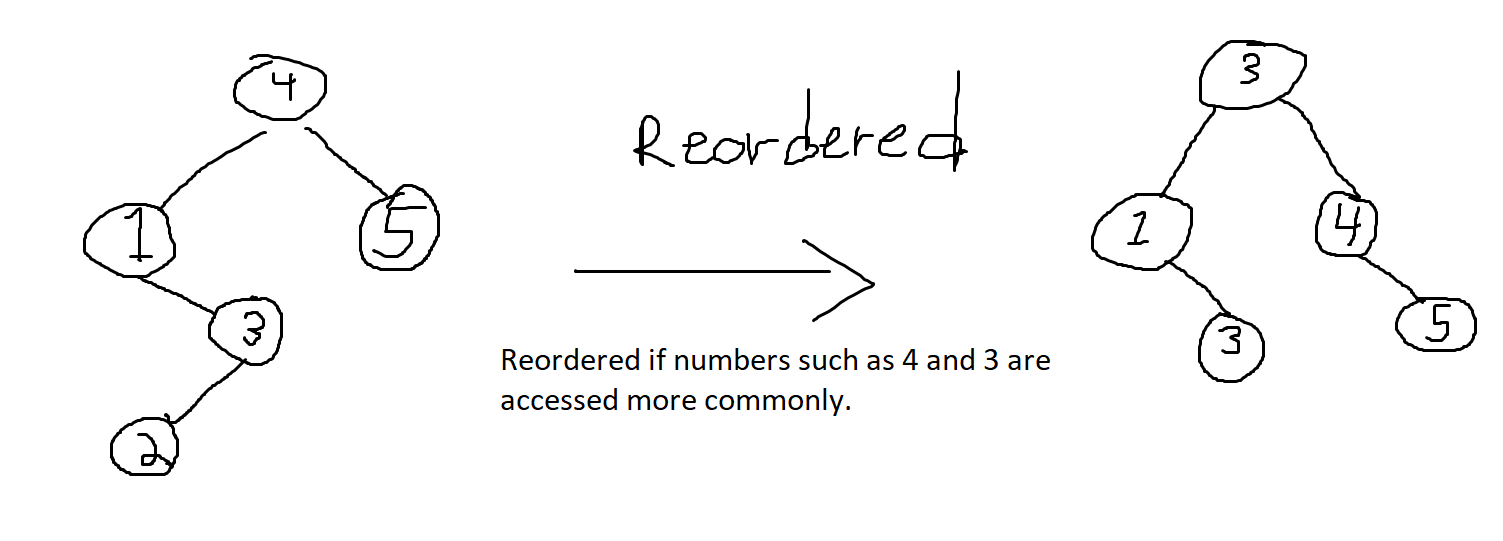
\includegraphics[scale=.35]{3.2.5.png}
\end{center}


\end{document}
